\documentclass[12pt]{article}

% for space filling
\usepackage{lipsum}
% highlighting hyper links
\usepackage[colorlinks=true, citecolor=blue]{hyperref}


%% meta data

\title{Example Paper}
\author{Luke Noel\\
  University of Connecticut
}

\begin{document}
\maketitle

\begin{abstract}
The abstract would go here. 
\end{abstract}

\section{Introduction}
\label{sec:intro}
Introduction to the paper.

% roadmap
The rest of the paper is organized as follows.
The data and equations will be presented in Section~\ref{sec:data}.
The methods are described in Section~\ref{sec:meth}.
The results are reported in Section~\ref{sec:resu}.
Appendix at the end in Section~\ref{sec:app}.

\section{Data}
\label{sec:data}

Write about the data here.

In line equation 1: $Z = (X - \mu)/\sigma$

In line equation 2: $y = 2*\pi$

\section{Methods}
\label{sec:meth}

Section to show methods you used. In display equation 1:
\begin{equation}
  \label{eq:exp}
  y = e^x,
\end{equation}

See Equation~\eqref{eq:exp} for natural exponential function.

In display equation 2:
\begin{equation}
  \label{eq:vol}
  (4/3)*\pi*r^3,
\end{equation}

See Equation~\eqref{eq:vol} for volume of a sphere formula.

section{Results}
\label{sec:resu}

Table~\ref{tab:car} shows first 5 rows of mtcars R dataset

\begin{table}[ht]
  \caption{Table 1 example}
  \label{tab:car}
\centering
\begin{tabular}{rrrrrrrrrrrr}
  \hline
 & mpg & cyl & disp & hp & drat & wt & qsec & vs & am & gear & carb \\ 
  \hline
Mazda RX4 & 21.00 & 6.00 & 160.00 & 110.00 & 3.90 & 2.62 & 16.46 & 0.00 & 1.00 & 4.00 & 4.00 \\ 
  Mazda RX4 Wag & 21.00 & 6.00 & 160.00 & 110.00 & 3.90 & 2.88 & 17.02 & 0.00 & 1.00 & 4.00 & 4.00 \\ 
  Datsun 710 & 22.80 & 4.00 & 108.00 & 93.00 & 3.85 & 2.32 & 18.61 & 1.00 & 1.00 & 4.00 & 1.00 \\ 
  Hornet 4 Drive & 21.40 & 6.00 & 258.00 & 110.00 & 3.08 & 3.21 & 19.44 & 1.00 & 0.00 & 3.00 & 1.00 \\ 
  Hornet Sportabout & 18.70 & 8.00 & 360.00 & 175.00 & 3.15 & 3.44 & 17.02 & 0.00 & 0.00 & 3.00 & 2.00 \\ 
   \hline
\end{tabular}
\end{table}

Figure~\ref{fig:iris} shows the sepal length vs. sepal width for the popular iris dataset in R.

\begin{figure}[ht]
  \centering
  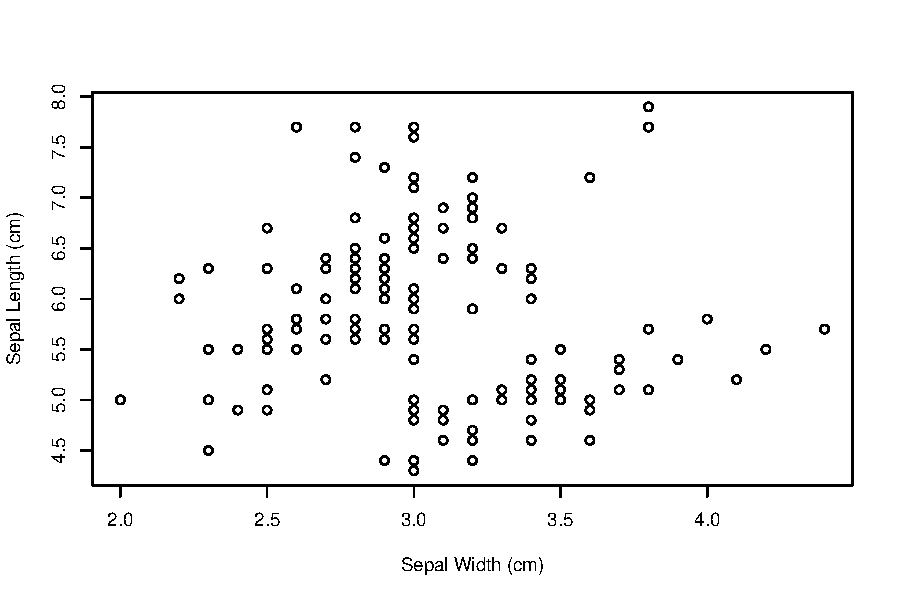
\includegraphics[width=\textwidth]{iris.pdf}
  \caption{Figure 1 example.}
  \label{fig:iris}
\end{figure}

